%%%% Proceedings format for most of ACM conferences (with the exceptions listed below) and all ICPS volumes.
\documentclass[sigconf]{acmart}

% \usepackage{amsmath}
%%%% As of March 2017, [siggraph] is no longer used. Please use sigconf (above) for SIGGRAPH conferences.

%%%% Proceedings format for SIGPLAN conferences 
% \documentclass[sigplan, anonymous, review]{acmart}

%%%% Proceedings format for SIGCHI conferences
% \documentclass[sigchi, review]{acmart}

%%%% To use the SIGCHI extended abstract template, please visit
% https://www.overleaf.com/read/zzzfqvkmrfzn

%%
%% \BibTeX command to typeset BibTeX logo in the docs
\AtBeginDocument{%
  \providecommand\BibTeX{{%
    \normalfont B\kern-0.5em{\scshape i\kern-0.25em b}\kern-0.8em\TeX}}}

%% Rights management information.  This information is sent to you
%% when you complete the rights form.  These commands have SAMPLE
%% values in them; it is your responsibility as an author to replace
%% the commands and values with those provided to you when you
%% complete the rights form.
\setcopyright{acmcopyright}
\copyrightyear{2019}
\acmYear{2019}
\acmDOI{10.1145/1122445.1122456}

%% These commands are for a PROCEEDINGS abstract or paper.
\acmConference[DocEng'19]{DocEng'19: ACM Symposium on Document Engineering}{September 23--26, 2019}{Berlin, DE}
% \acmBooktitle{Woodstock '18: ACM Symposium on Neural Gaze Detection, June 03--05, 2018, Woodstock, NY}
% \acmPrice{15.00}
% \acmISBN{978-1-4503-9999-9/18/06}


%%
%% Submission ID.
%% Use this when submitting an article to a sponsored event. You'll
%% receive a unique submission ID from the organizers
%% of the event, and this ID should be used as the parameter to this command.
%%\acmSubmissionID{123-A56-BU3}

%%
%% The majority of ACM publications use numbered citations and
%% references.  The command \citestyle{authoryear} switches to the
%% "author year" style.
%%
%% If you are preparing content for an event
%% sponsored by ACM SIGGRAPH, you must use the "author year" style of
%% citations and references.
%% Uncommenting
%% the next command will enable that style.
%%\citestyle{acmauthoryear}

%%
%% end of the preamble, start of the body of the document source.
\begin{document}

%%
%% The "title" command has an optional parameter,
%% allowing the author to define a "short title" to be used in page headers.
\title{Automatic Identification and Normalisation of Physical Measurements in Scientific Literature}

%%
%% The "author" command and its associated commands are used to define
%% the authors and their affiliations.
%% Of note is the shared affiliation of the first two authors, and the
%% "authornote" and "authornotemark" commands
%% used to denote shared contribution to the research.
\author{Luca Foppiano}
\email{FOPPIANO.Luca@nims.go.jp}
\orcid{0000-0002-6114-6164}
\affiliation{%
  \institution{National Institute for Materials Science (NIMS)}
  \streetaddress{1-2-1 Sengen}
  \city{Tsukuba}
  \postcode{305-0047}
  \country{Japan}
}

\author{Laurent Romary}
\email{laurent.romary@inria.fr}
\orcid{0000-0002-0756-0508}
\affiliation{
  \institution{Inria}
  \streetaddress{2 Simone Iff}
  \city{Paris}
  \postcode{75012}
  \country{France}
}

\author{Masashi Ishii}
\email{ISHII.Masashi@nims.go.jp}
\orcid{0000-0003-0357-2832}
\affiliation{%
  \institution{National Institute for Materials Science (NIMS)}
  \streetaddress{1-2-1 Sengen}
  \city{Tsukuba}
  \postcode{305-0047}
  \country{Japan}
}

\author{Mikiko Tanifuji}
\email{TANIFUJI.Mikiko@nims.go.jp}
\orcid{000-0001-5284-6364}
\affiliation{%
  \institution{National Institute for Materials Science (NIMS)}
  \streetaddress{1-2-1 Sengen}
  \city{Tsukuba}
  \postcode{305-0047}
  \country{Japan}
}

%%
%% By default, the full list of authors will be used in the page
%% headers. Often, this list is too long, and will overlap
%% other information printed in the page headers. This command allows
%% the author to define a more concise list
%% of authors' names for this purpose.
\renewcommand{\shortauthors}{Foppiano, et al.}

%%
%% The abstract is a short summary of the work to be presented in the
%% article.
\begin{abstract}
We present Grobid-quantities, an open source application for parsing and normalising measurements from scientific and patent literature~\cite{grobid-quantities}. Tools of this kind represent the building blocks for large-scale Text and Data Mining (TDM) systems whose goal is to understand and make unstructured information accessible through standardised methods. 
Grobid-quantities is a module built up on top of Grobid~\cite{GROBID}, a machine learning framework for parsing and structuring PDF documents. Designed to process large quantities of data, it provides a robust implementation in batch mode or via a REST API. The machine learning engine architecture follows the cascade approach, where each model is specialised in the resolution of a specific task. The models are trained using a CRF (Conditional Random Field) algorithm for extracting quantities (atomic values, intervals or lists), units (such as length, weight) and different value representations (such as alphanumeric, power of 10, exponential). Identified measurements are normalised according to the International System of Units (SI)~\cite{internationalSystemOfUnits}. 
Thanks to its consistent recall and reliable precision, Grobid-quantities has been integrated as a measurement-extraction engine in various TDM projects, such as Marve (Measurement Context Extraction from Text)~\cite{hundman2017measurement}, for extracting semantic measurements and meaning in Earth Science. At the National Institute for Materials Science (NIMS), a project for application of Grobid-quantities to discover new superconducting materials is in progress: normalised materials characteristics extracted from scientific literature are a key resource for materials informatics (MI)~\cite{foppiano2019proposal}. 
\end{abstract}

%%
%% The code below is generated by the tool at http://dl.acm.org/ccs.cfm.
%% Please copy and paste the code instead of the example below.
%%
 \begin{CCSXML}
<ccs2012>
<concept>
<concept_id>10010405.10010497.10010504.10010505</concept_id>
<concept_desc>Applied computing~Document analysis</concept_desc>
<concept_significance>500</concept_significance>
</concept>
<concept>
<concept_id>10010405.10010497.10010500.10010503</concept_id>
<concept_desc>Applied computing~Document metadata</concept_desc>
<concept_significance>300</concept_significance>
</concept>
<concept>
<concept_id>10010405.10010497.10010510.10010514</concept_id>
<concept_desc>Applied computing~Format and notation</concept_desc>
<concept_significance>300</concept_significance>
</concept>
</ccs2012>
\end{CCSXML}

\ccsdesc[500]{Applied computing~Document analysis}
\ccsdesc[300]{Applied computing~Document metadata}
\ccsdesc[300]{Applied computing~Format and notation}

%%
%% Keywords. The author(s) should pick words that accurately describe
%% the work being presented. Separate the keywords with commas.
\keywords{machine learning, tdm, measurements, physical quantities}

%%
%% This command processes the author and affiliation and title
%% information and builds the first part of the formatted document.
\maketitle

\section{Introduction}

The data overflow in scientific publications is a widely known challenge impacting the accessibility to relevant information for both researchers and readers. 
%The amount of data that a single scientist might be dealing with tend to be overwhelming because understanding requires to spend many hours (re-)reading a single article to grasp its message and significance. It's simply too much for a single human to keep up with the new fresh information that is available daily. 
%Luckily technology has evolved: advances in natural language processing (NLP) in combination with Deep Neural Network have reached results above average human precision. 
%Motivation
One of the core elements of science is the physical quantity or measurement, which combine quantification of units (such as grams or micrometers). The automatic extraction of measurements has been studied for many years. Nowadays, despite the technology has evolved, there are still several challenges to overcome: (1) natural language and writing style introduce additional variability (for example length can be expressed as m, meter, metre). Overlaps (2) between different unit of measurements (like inductance \textit{pico Henry} and acidity share the same notation \textit{pH}). The ability correctly create new knowledge bases from physical measurements can foster the creation of advanced search services. 

%Grobid-quantities
In this paper, we present Grobid-quantity, an Open Source application \cite{grobid-quantities} for parsing and normalising measurements from scientific and patent literature. Using the machine learning (ML) CRF (Conditional Random Field) algorithm, it provides a framework for extracting quantities (atomic values, ranges, intervals and lists), units (like length, weight) and different value representations (such as alphanumeric, power of 10, exponential). Identified measurements are then normalised or transformed toward the International System of Units (SI). Thanks to its high recall and reliable precision, Grobid-quantities has been integrated as a measurement-extraction engine in various TDM projects \cite{foppiano2019proposal}.

This article is organised as follow. In Section \ref{sec:related_work} we discuss the related work. Then, we describe the system in Section \ref{sec:system} and we provide the evaluation and use cases in Sections \ref{sec:results} and  \ref{sec:use_cases}. Finally, we conclude the article in Section \ref{sec:conclusion}.

\section{Related Work}
\label{sec:related_work}
Previous attempts to extract measurements from text have been made previously. Often rely on rule-based systems or formal grammars, combining handwritten rules with look-ups in terminological databases.  

Quantalyze, a commercial tool, was reported by  \cite{hundman2017measurement} showing weak recall and covering a subset of units \cite{aras2014applications}. Another experimental approach using GATE (General Architecture for Text Engineering), described in \cite{agatonovic2008large}, addressed the identification of numeric properties from patents. \cite{am2013processing} investigated issues applied to Russian-derived languages. These approaches lack either the generalisation to an extensive corpus or deal mainly with a specific languages. \cite{berrahou2013extract} described an attempt to recognise units using machine learning in combination with pattern matching and string distance to an ontology. \cite{kang_extracting_2013} describe another ML-based approach focusing on experimental results restricted to biological domain. Our work differs because it recognises units and various type of quantitative values. Our extraction is fully ML-based and includes a normalisation process toward the International System of Units (SI). 

\section{System description}
\label{sec:system}
Grobid-quantities is a Java application, based on Grobid framework (GeneRation Of BIbliographic Data)~\cite{GROBID}. Using the low-level Grobid abstraction can structure and manipulate PDFs natively. It supports large-scale processing via batch or web REST API. The front-end provides a visualisation module to show extracted measurements on PDF.

\subsection{Data model}
\label{subsub:data-model}
\begin{figure}[ht]
  \centering
  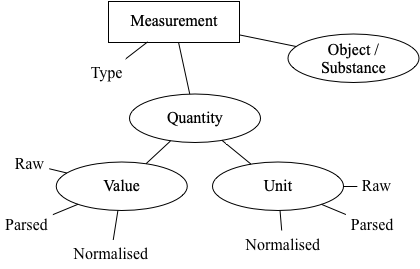
\includegraphics[width=\linewidth]{images/schema-2}
  \caption{Data model schema}
  \label{fig:data-model-schema-2}
  \Description{Data model schema}
\end{figure}
We define \textit{Measurement} the association of an object or a substance with one or more \textit{quantities}, depending on a \textit{type}. (a) atomic, in case of a punctual measurement (10 grams). (b) interval (\textit{from 3 to 5 mmol}) and (c) range ($100 \pm 4$), when the quantification covers continuous values. Finally, (d) list of discrete values of the same quantity. A \textit{Quantity} link a  quantitative value and an (optional) unit (Figure~\ref{fig:data-model-schema-2}). 
When dealing with text extracted from PDFs there is a relevant amount of noise that needs to be handled (spaces, wrong UTF-8 characters, missing fonts). Therefore, we designed this model to allow return of partial results: the \textit{Value} and \textit{Unit} entities allows three different representation fo the same information: \textit{raw} as appear in text, \textit{parsed} when they are converted to the logical (number) representation and finally \textit{normalised} when they are converted to the equivalent base unit in the SI system. 

Values can be of five types: numeric (2, 1000), alphanumeric (two, thousand), power of 10 ($3\cdot10\textsuperscript{5}$) and exponential representation using the mathematical constant e = 2.2718 ($0.2\cdot e\textsuperscript{3}$), dates are also expressions of measurements of time. Units objects are more complex to manage because of several measurement systems. For simplicity we modelled them following the SI system which allows representing units as products of simpler compounds: we trained ML models to transform m/s to their product representation $m \cdot s\textsuperscript{-1}$.

\subsection{Architecture}
The system takes in input text or PDF and performs three steps: (a) tokenisation, (b) measurement extraction and parsing and (c) quantity normalisation. 

\subsubsection{Tokenisation}
The tokenisation is the process of splitting input data in tokens. Grobid-quantities uses a two-phase tokenisation, first by punctuation, then each resulting token is re-tokenised using a regex aiming to separate sequential digits and alphanumeric characters. Given the example 25m\^2, first passage returns ["25m","\^","2"] and the second ["25","m","\^","2"]. 

\subsubsection{Extraction}
The extraction is composed by three CRF (Conditional Random Field) models applied in cascade: \textit{Quantities}, \textit{Units} and \textit{Values} (Figure \ref{fig:schema-cascade}). 

\begin{figure}[ht]
  \centering
  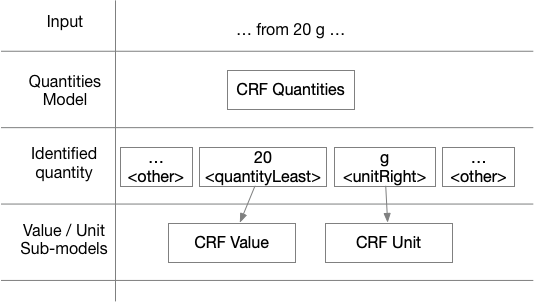
\includegraphics[width=\linewidth]{images/schema-cascade}
  \caption{Illustrate the cascade approach in applying CRF models. The input is first parsed by the Quantities model, which recognise the type of measurement (list, ranges, interval and atomic values) and units. They are then passed to further CRF sub-models: in this case Values and Units respectively.}
  \label{fig:schema-cascade}
  \Description{Illustrate the cascade approach in applying CRF models. The input is first parsed by the Quantities model, which recognise the type of measurement (list, ranges, interval and atomic values) and units. They are then passed to further CRF sub-models: in this case Values and Units respectively.}
\end{figure}

% Quantity model 
The \textit{Quantities} CRF model takes in input a sequence tokens identify quantities as combination of units and values \ref{tab:quantities-model-labels}. The process requires additional labels defining positional information (such as <unitLeft>, <unitRight> for units) because of the lack of structure in sequence labelling output. 

\begin{table}[ht]
  \caption{Labels description for the CRF model for Quantities. In bold the token the label refers to.}
  \label{tab:quantities-model-labels}
  \begin{tabular}{lll}
    \toprule
    Label & Description & Example\\
    \midrule
    <valueAtomic> & value of an atomic quantity & \textbf{2} m \\
    <valueLeast> & least value in an interval & from \textbf{2} m \\
    <valueMost> & max value in an interval & up to \textbf{7} m \\
    <valueBase> & base value in a range & $\textbf{20}\pm7$ m \\
    <valueRange> & range value in a range & $20 \pm \textbf{7}$ m \\
    <valueList> & list of quantities & \textbf{2}, \textbf{3} and \textbf{10} m \\
    <unitLeft> & left-attached unit & \textbf{pH} 2 \\
    <unitRight> & right-attached unit & 2 \textbf{m} \\
    <other> & everything else & - \\
  \bottomrule
\end{tabular}
\end{table}

% Gazetteers
Previous works (described in Section \ref{sec:related_work}) made extensive use of gazetteers (database, ontology) to improve performances. We compiled a list of units (localised in English, French and German) with their main characteristics: system (SI base, SI derived, imperial, ...) and type (volume, length, ...). Their representations: notations (m\textsuperscript{3}, m\^3), lemmas (cubic meter, cubic metre) and inflections (cubic meters, cubic metres).  We made this list available through the \textit{Unit lexicon} by providing units lookups by properties (notation, lemma, inflexion, and so forth). A second gazetteer was created to allow the transformation of alphabetic values in numeric ones (for example, twenty-one to 21).

The \textit{Quantities} CRF model uses standard lexical information and orthogonal features obtained by the \textit{Unit lexicon}, indicating  whether a token is a known unit. Layout information (such as formatting, subscript or superscript) are not used. The resulting units and values are processed in cascade by the respective models. 

% Unit model 
The \textit{Units} CRF model works at character level and uses the \textit{Unit lexicon} for orthogonal features. It parses a unit in a list of product of triples (prefix, base, power) (Table \ref{tab:units-model-labels}). For example Kg/mm\textsuperscript{2} can be transformed as [(K, g, 1), (m, m, -2)]. Units outside the SI (e.g. miles) are transformed in a single product with only the "base" element ([(,mile,)]). 

\begin{table}[ht]
  \caption{Labels description for the CRF model for Units. The example shows in bold the part referred by the label. }
  \label{tab:units-model-labels}
  \begin{tabular}{lll}
    \toprule
    Label & Description & Example\\
    \midrule
    <prefix> & prefix of the unit  & \textbf{k}g\textsuperscript{2} \\
    <base> & unit base & k\textbf{g}\textsuperscript{2}\\
    <pow> & unit power & kg\textsuperscript{\textbf{2}}\\
    <other> & everything else & - \\
  \bottomrule
\end{tabular}
\end{table}

We use the products of triples to create well-formatted units and use them to fetch complementary information (system, type) from the \textit{Unit lexicon}. Let's suppose the raw text contains "10 m 3". The Quantity model identifies 10 as atomic value and "m 3" as the unit. The Unit model identifies "m" as the base and "3" as power: [(,m,3)]. This product is then reformatted as "m\^3" and looked up in the gazetteer. Since "m\^3" exists, system=SI, inflection='Cubic meters' and type=volume are attached to the unit object. 

% Value model 
The \textit{Values} model processes any identified values. It supports five types: numeric, alphabetic, power-10, exponential, and time expression (Table \ref{tab:values-model-labels}). Each type is parsed in a different way: alphabetic expressions are looked up in the word-to-number gazetteer, power-10 and exponential are calculated mathematically. Time expressions are processed using the built-in Date model from Grobid \cite{GROBID}.

\begin{table}[ht]
  \caption{Labels description for the CRF model for Values. In bold an example of token the specific label recognise.}
  \label{tab:values-model-labels}
  \begin{tabular}{lll}
    \toprule
    Label & Description & Example\\
    \midrule
    <number> & numeric value & $\textbf{2.5}\cdot10\textsuperscript{\textbf{5}}$ \\
    <alpha> & alphabetic value & \textbf{twenty} \\
    <time> & time expression  & in \textbf{1970-01-02}\\
    <exp> & exponential expression & $0.2\cdot\textbf{e}\textsuperscript{3}$ \\
    <base> & base of the power expression & $2.5\cdot\textbf{10}\textsuperscript{5}$\\
    <pow> & power in a power expression & $2.5\cdot10\textsuperscript{\textbf{5}}$ \\
    <other> & everything else & - \\
  \bottomrule
\end{tabular}
\end{table}

\subsubsection{Normalisation}

The normalisation is the final step of the chain where all the measurement with a valid parsed value are transformed to the base SI unit (grams to kg, Celsius to Kelvin, and so on). Since the normalisation process may fail for multiple reasons, errors are reported but ignored for the sake of the processing. We use an external Java library called Units of Measurement~\cite{units_of_measurement} which provides a set of interfaces and implementations for safely handling units and quantities. Dealing with measurement transformation lead often to common mistakes due rounding and wrong approximations. At the time this paper is being written, the final revised version of this library is accepted under the Java Standardisation Process JSR-385\footnote{\url{https://jcp.org/en/jsr/results?id=6096}}. 

\section{Evaluation and results}
\label{sec:results}

We trained and evaluated the system using a corpus of 32 randomly selected Open Access (OA) English articles from different domains such as medicine, robotics, astronomy, physiology. We have also included three patents translated in English, French and German. Three people annotated the corpus and each document was cross-checked. We partition training and evaluation data using 80/20 proportion. After training, we estimated precision, recall and F1-score for each model, using the evaluation framework built-in in Grobid. These measure indices are calculated at three different levels: token-level, field-level and instance-level. Consider a sequence of tokens with their predicted and expected labels. While token-level scores are calculated independently for each token, field-level scores are calculated for each continuous sequence of tokens under the same label (so a field, a sequence of several tokens which all belong to the same labelled chunk, e.g. an unit), finally instance level is the score for the whole input, for instance a paragraph~\cite{foppiano2019proposal}. 

\begin{table}[ht]
   \caption{Quantities CRF model evaluation results (precision, recall and F1-score).}
   \label{tab:quantities-evaluation}
   \begin{tabular}{c|ccc|ccc}
       \toprule
       Label & \multicolumn{3}{c}{\textbf{Token-level}} & \multicolumn{3}{c}{\textbf{Field-level}}\\
        & P & R & F1 & P & R & F1 \\
       \midrule
       <unitLeft>    & 98.94 & 95.23 & 97.05 & 97.8  & 95.11 & 96.43\\
       <unitRight>   & 66.67 & 66.67 & 66.67 & 59.09 & 54.17 & 56.52\\
       <valueAtomic> & 86.63 & 87.81 & 87.22 & 87.39 & 87.17 & 87.28\\
       <valueBase>   & 95.12 & 100   & 97.5  & 94.12 & 94.12 & 94.12\\
       <valueLeast>  & 82.81 & 65.43 & 73.1  & 81.89 & 67.1  & 73.76\\
       <valueList>   & 77.69 & 56.63 & 65.51 & 76.06 & 58.06 & 65.85\\
       <valueMost>   & 78.05 & 73.44 & 75.68 & 81.68 & 64.46 & 72.05\\
       <valueRange>  & 96.67 & 100   & 98.31 & 94.44 & 94.44 & 94.44\\
       \midrule
       average       & 88.81  & 85.08 & \textbf{86.9} & 89.59 & 84.6 & \textbf{87.02}\\
       \bottomrule
   \end{tabular}
\end{table}

As shown in Tables \ref{tab:quantities-evaluation} we obtain average F1-score of 86.9\% and 87.01\% for token and field-level respectively. The low results for \textit{<valueLists>} and \textit{<unitRight>} suggests that more examples of that kind are required. Simple pattern structure and lower expression variability can explain the high f1-score for \textit{<valueRange>} as compared with \textit{<valueAtomic>} or \textit{<valueLeast>}. The recall at instance level is 68.49\%, indicating that more than half of the evaluated paragraphs contained no errors. 

\begin{table}[ht]
    \caption{Units CRF model evaluation results (precision, recall and F1-score).}
    \label{tab:units-evaluation}
    \begin{tabular}{c|ccc|ccc}
        \toprule
        Label & \multicolumn{3}{c}{\textbf{Token-level}} & \multicolumn{3}{c}{\textbf{Field-level}}\\
        & P & R & F1 & P & R & F1 \\
        \midrule
        <base>    & 97.52 & 92.49 & 94.94 & 77    & 82.8  & 79.79 \\
        <pow>     & 81.82 & 90    & 85.71 & 73.33 & 84.62 & 78.57 \\
        <prefix>  & 62.79 & 93.1  & 75    & 70.27 & 92.86 & 80    \\
        \midrule
        average   & 90.64  & 92.37 & \textbf{91.49} & 75   & 85.07 & \textbf{79.72} \\
        \bottomrule
   \end{tabular}
\end{table}

Table \ref{tab:units-evaluation} shows that \textit{Units} CRF models f1-score is 91.49\% and 79.72\% for token and instance level respectively. We notice the model tend to have lower results for \textit{<prefix>} label; intuitively this can be due to overlaps with \textit{<base>}. The instance-level recall is consistently high at 85.06\%. 

\begin{table}[ht]
  \caption{Values CRF model evaluation results (precision, recall and F1-score).}
  \label{tab:values-evaluation}
  \begin{tabular}{c|ccc|ccc}
    \toprule
    Label & \multicolumn{3}{c}{\textbf{Token-level}} & \multicolumn{3}{c}{\textbf{Field-level}}\\
    & P & R & F1 & P & R & F1 \\
    \midrule
    <alpha>       & 100   & 100   & 100   & 96.74 & 99.44 & 98.07   \\
    <base>        & 66.67 & 42.86 & 52.17 & 90    & 90    & 90      \\
    <number>      & 90.43 & 97.2  & 93.69 & 96.95 & 98.07 & 97.5    \\
    <pow>         & 77.78 & 50    & 60.87 & 80    & 80    & 80      \\
    <time>        & 54.55 & 75    & 63.16 & 57.69 & 83.33 & 68.18   \\
    \midrule
    average       & 91.85 & 90.95 & \textbf{91.4} & 86.18 & 86.75 & \textbf{86.47}   \\
    \bottomrule
     \end{tabular}
\end{table}

Finally \ref{tab:values-evaluation} indicate Values CRF model average f1-score of 91.4\% and 86.47\% for token and field level respectively. Low precision for \textit{<base>} can be explained caused by overlaps with other labels, as for the  \textit{Units} model. Recall at instance-level is 90.23\%.  

Thanks to these results, Grobid-quantities provided prospects to be employed in more extensive system for automatic Text and Data Mining. 

\section{Use cases}
\label{sec:use_cases}
\cite{hundman2017measurement} described a system for extracting semantic measurements and meaning in Earth Science, Marve (Measurement Context Extraction from Text), using Grobid-quantities in combination with their approach based on dependency parsing. The ISTEX~\cite{dazy2014istex} project financed a pilot project to evaluate the applicability of extracted measurement to a enhanced information retrieval system, where document can be found by measurement search. Recently, the normalised data extraction is strongly required in materials research, because an inverse problem in which high performance materials are predicted from properties is expected to be solved with well-organised big data. At the National Institute for Materials Science (NIMS), a project to discover new superconducting materials is in progress. The system being developed relays on Grobid-quantities which can extract and normalise superconducting properties such as critical temperature (Tc) with units of mK and K and critical pressure expressed with units of Pa, MPa, and GPa in scientific literature ~\cite{foppiano2019proposal}. 

% Istex, Marve, NIMS
\section{Conclusion}
\label{sec:conclusion}
In this paper, we presented Grobid-quantities, a system for extracting and normalising measurement from scientific literature. Results are encouraging so that the system can be used, although there is still needs to have more training data, in particular for the \textit{Quantities} CRF model. The integration of Grobid-quantities in other projects suggests maturity from the engineering point of view. In the next steps, we plan to introduce deep neural networks like Bi-LSTM+CRF approach and embeddings as replacement to the statistical CRF models. 

%%
%% The acknowledgements section is defined using the "acks" environment
%% (and NOT an unnumbered section). This ensures the proper
%% identification of the section in the article metadata, and the
%% consistent spelling of the heading.
\begin{acks}
Our warmest thanks to Patrice Lopez, who initiated and supported Grobid-quantities, author of Grobid~\cite{GROBID} and many other Open Source TDM tools. Thanks our colleagues at NIMS Thaer M. Dieb, and Akira Suzuki for the support received. Finally, thanks to Units of Measurements's contributors\footnote{https://github.com/orgs/unitsofmeasurement/people}.
\end{acks}

%%
%% The next two lines define the bibliography style to be used, and
%% the bibliography file.
\bibliographystyle{ACM-Reference-Format}
\bibliography{references}

%%
%% If your work has an appendix, this is the place to put it.
% \appendix

\end{document}
\endinput
%%
%% End of file `sample-sigconf.tex'.
